\subsection{Linear Separability}

As stated before, a perecptron is a binary classifier. A fairly obvious application of the concept is for classification. There are several instances where classification is necessary. \\
		
		For this report, we have chosen a rudimentary example of a classification task: \textbf{Linear separability}. Consider a set of blue points and a set of red points on a two-dimensional plane. The two sets are linearly separable if there exists a line on the plane such that all of the blue points lie on one side of the plane and all of the red points lie on the other side. \\

\begin{center}
	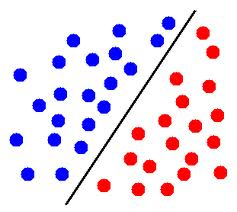
\includegraphics[scale=0.5]{ls}
\end{center}

Shown above is an instance of two-dimensional linear separation. This idea is immediately generalized to n-dimensional Euclidean spaces if the line is replaced by a hyperplane.

\subsection{How is the Perceptron useful here?}
Recall that a Perceptron accepts a set of inputs and produces an output of either 0 or 1. We can pass in the coordinates of each point along with the bias (which we will explain later) and the expected output. This will be a $4x1$ column vector. We will call our input vector $x$. \\

	\begin{center}
		$x = 
		\begin{bmatrix}
			b \\
			i1 \\
			i2 \\
			y
		\end{bmatrix}
		$
	\end{center}

where $b$ is the bias, $i1$ is the x-coordinate of the point, $i2$ the y-coordinate, and $y$ is the expected output (0 or 1). \\

\subsection{Implementing the Perceptron}
We decided to use Python to implement the algorithm. We generated 10 random two-dimensional points such that they are linearly separable. \\

	\begin{center}
		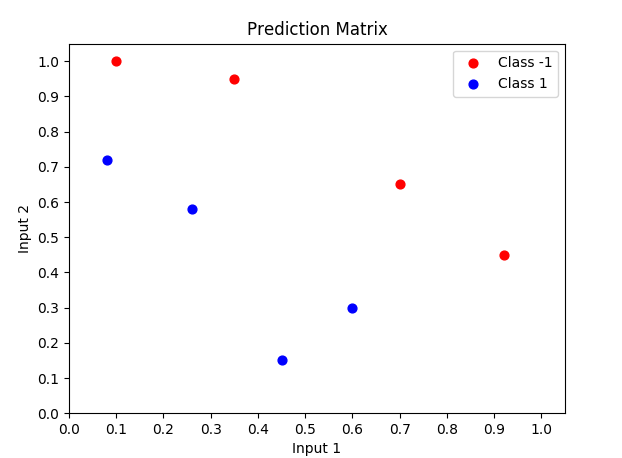
\includegraphics[scale=0.5]{pts}
	\end{center}
	
Shown above is are the 10 points plotted. Notice how there is a line (with slope $\approx$ -1) that can separate the two sets. The points above the line will be Class -1 and have a color of Red, while the points below the line will be Class 1 and have a color of Blue. \\

We will first implement a function $predict()$ that will return the appropriate class for a specified set of inputs and their corresponding weights. \\


	\begin{lstlisting}[language=Python, frame=single]
# Returns 1 if the weighted input sum is greater 
# than a threshold.
def predict(inputs, weights):
    activation_threshold = 0.0

    # Obtaining the weighted sum of the inputs.
    for i, w in zip(inputs, weights):
        activation_threshold += w * i

    return 1.0 if activation_threshold >= 0.0 else 0.0
	\end{lstlisting}
	
This function takes in the input vector and its corresponding weights as arguments. We loop through the vectors (which are called arrays in Python) and calculate the weighted sum of the inputs. In this case, our threshold is 0. If the weighted sum is positive (Class 1) we return 1. If not (Class -1), we return 0. This will help us calculate the error in prediction (explained later). \\

NOTE: In the $main()$ function, we will have a $3x1$ vector called $weights$ that will be modified during each iteration of the training using backpropogation. \\

Next, we implement a function $accuracy()$ that will calculate the percentage accuracy of the classifier during each iteration. \\ 

	\begin{lstlisting}[language=Python, frame=single]
# Returns the percentage accuracy of the classifier.
def accuracy(matrix, weights):
    num_correct = 0.0
    preds = []

    for i in range(len(matrix)):
        pred = predict(matrix[i][:-1], weights)
        preds.append(pred)

        if pred == matrix[i][-1]:
            num_correct += 1.0

    print("Predictions:", preds)

    return num_correct / float(len(matrix))
	\end{lstlisting}
	
This function takes in a two dimensional array (a matrix) and a vector of weights. We loop through the two-dimensional array (through all the data vectors) and in each iteration, call the $predict()$ function to obtain the prediction for each data vector's class. We check to see if the predicted class is the same as the expected class. If it is, then we increment the counter by 1. At the end of the function, we return a decimal representation of the accuracy. \\

	\begin{lstlisting}[language=Python, frame=single]
# Backpropogation algorithm
def train_weights(matrix, weights, n_epoch=10, 
l_rate=1.00, do_plot=False, stop_early=True, 
verbose=True):

    for epoch in range(n_epoch):
        current_accuracy = accuracy(matrix, weights)
        print("\nEpoch %d \nWeights: " %epoch, weights)
        print("Accuracy: ", current_accuracy)

        # If the maximum accuracy is reached
        if current_accuracy == 1.0 and stop_early:
            break

		# 
        if do_plot:
            plot(matrix, weights, title="Epoch %d" 
            %epoch)

        for i in range(len(matrix)):

            # Current prediction
            prediction = predict(matrix[i][:-1], 
            weights)

            # Error in prediction
            error = matrix[i][-1] - prediction

            # Updating the weights
            for j in range(len(weights)):
                if verbose:
                    sys.stdout
                    .write("\tWeight[%d]: %0.5f --> "
                    %(j, weights[j]))

                # Updating the weights.
                weights[j] += 
                (l_rate * error * matrix[i][j])

                if verbose:
                    sys.stdout
                    .write("%0.5f\n"
                    %(weights[j]))
    
    # Plotting the final matrix.
    plot(matrix, weights, title="Final epoch")
    return weights
	\end{lstlisting}